\chapter{Basic definitions}

\begin{defn}
	\textbf{Matroid} $\M = (E, \I)$ is for $E$ finite non-empty set and $\I \subseteq 2^E$ (also called as independent sets) satisfying these properties:
	
	\begin{enumerate}[(\text{I}1)]
		\item $\emptyset \in \I$,
		\item $I \in \I \Rightarrow \forall I' \subseteq I : I' \in \I$,
		\item $I_1, I_2 \in \I, \abs{I_1} < \abs{I_2} \Rightarrow \exists e \in I_2 \setminus I_1: I_1 \cup \{e\} \in \I$.
	\end{enumerate}
\end{defn}

\begin{notation}
	For further use and simplification we will sometimes use $I + e$ as a substitution for $I \cup \{e\}$. Similarly also $I - e$ for $I \setminus \{e\}$.
\end{notation}

\begin{example}
	For a given multi-graph $G = (V,F)$ we will set $E = F$ (or in other words $E$ stands for edges and the set). Independent sets $\I$ will be all acyclic subsets of $E$. Easily seen (I1) and (I2) is satisfied. For the third one (I3) it is also quite easily seen, because if we have one larger and smaller non-cycles then we can append one edge from the larger to the smaller.
\end{example}

\begin{example}
	Let $E$ be some elements of a vector space $V$. If $X \subseteq E$ is independent then it is linearly independent in $V$.
\end{example}

\begin{defn}
	Matroid \textbf{isomorphism} for two matroids $\M_i = (E_i, \I_i)$ for $i = 1,2$ is a bijection $f: E_1 \to E_2$ satisfying $\forall X \subseteq E_i : X \in \I_1 \Leftrightarrow f(X) \in \I_2$.
\end{defn}

\section{Circuits}

\begin{defn}
	$X \subseteq E$ is a \textbf{circuit} if $X \notin \I$ and $\forall x \in X : X - x \in \I$. Also we will denote $\C(\M)$ as the set of all circuits of $\M$.
\end{defn}

\begin{lemma}
	Let $\M = (E, \I)$ be a matroid and $\C$ its collection of circuits, then
	
	\begin{enumerate}[(C1)]
		\item $\emptyset \notin \C$,
		\item $\forall C_1, C_2 \in \C : C_1 \subseteq C_2 \Rightarrow C_1 = C_2$ and
		\item $C_1, C_2 \in \C, C_1 \neq C_2, e \in C_1 \cap C_2 \Rightarrow C_3 \subseteq (C_1 \cup C_2) -e , C_e \in \C$.
	\end{enumerate}
\end{lemma}

\begin{proof}
	(C1) and (C2) are easily seen from (I1) and (I2). Now for the third part (C3). So for contradiction let $C_1, C_2, e$ be as mentioned in the first part, but $(C_1 \cup C_2) - e \in \I$. Then $\exists f \in C_2 \setminus C_1 : C_2 - f \in \I$. Now find $I \in \I$ max s.t. $C_2 \setminus \{f\} \subseteq I \subseteq C_1 \cup C_2$. If $f \notin I$ then it would contain $C_2$ which is dependent and $\exists g \in C_1 \setminus C_2 : g \notin I$ otherwise it would contain $C_1$ which is dependent. Therefore
	
	$$
	|I| \leq | C_1 \cup C_2 | - 2 < |(C_1 \cup C_2) - e|
	$$
	
	\noindent and now we may use the third axiom (I3) that is $\exists x \in |(C_1 \cup C_2) - e| \setminus I$ s.t. $I + e \in \I$ (this cannot be otherwise $I$ contains the whole $C_2$). Now $I + x$ contradicts the maximality of $I$.
\end{proof}

\begin{claim}
	Lets have $E$ and $\C \subseteq 2^E$ satisfying all (C1), (C2) and (C3). Then set $\I = \{X \subseteq E | \forall C \in \C : C \nsubseteq X\}$ and $\M = (E, \I)$ is a matroid.
\end{claim}

\begin{proof}
	We have to show all properties of matroid. That is (I1) is trivially satisfied and (I2) also trivially holds. For the last (I3) we use a contradiction. For that we have $I_1, I_2 \in \I$, then $\forall e \in I_2 \setminus I_1 : I_1 + e \notin \I$. Let $I_3 \subseteq I_1 \cup I_2$ s.t. $|I_3| > |I_1|$ and $|I_1 \setminus I_3|$ is minimal. If $|I_1 \setminus I_3|$ would be empty then (I3) will hold, therefore assume it is non-empty.
	
	Fix $e \in I_1 \setminus I_3$. Let $I_k = |I_3 - f| +e$ for $(f \in I_3 \setminus I_1)$. This cannot be independent ($\notin \I$) therefore $\exists C_k \subseteq T_k : C_k \in \C$ and $f \notin C_k, e \in C_k$.
	
	$(I_3 \setminus I_1) \cap C_k = \emptyset$ hence $C_k \subseteq T_k \setminus (I_3 \setminus I_1) = (I_1 \cap I_3) + e \subseteq I_1$ this is not possible so it must be non-empty. Then $\exists g \in (I_3 \setminus I_1) \cap C_k \Rightarrow C_k, C_g \in \C, e \in C_k \cap C_g, f \notin C_k, g \notin C_g$ but $(C_k \cup C_g) - e \subseteq I_3$ which is contradiction with (C3).
\end{proof}

\section{Basis}

\begin{defn}
	Let $\M = (E, \I)$ be a matroid. Then $B$ is a \textbf{basis} iff $B \in \I, \forall x \in E \setminus B: B + x \notin \I$.
\end{defn}

\begin{prop}
	Let $B_1, B_2$ be bases of $\M$, then $\abs{B_1} = \abs{B_2}$.
\end{prop}

\begin{proof}
	If $|B_1| < |B_2|$ then by (I3) $\exists x \in B_2 \setminus B_1 : B_1 + x \in \I$.
\end{proof}

\begin{defn}
	Let $\B (\M) = \{B \subseteq E , B \text{ is a basis}\}$ be a collection of basis satisfying
	
	\begin{enumerate}[(B1)]
		\item $\B \neq \emptyset$ and
		\item $B_1, B_2 \in \B, e \in B_1 \setminus B_2 \Rightarrow \exists f \in B_2 \setminus B_1 : |B_1 - e| + f \in \B$.
	\end{enumerate}
\end{defn}

One can see that (B2) can be proven using $I_1 - e =: B_1$ and $I_2 = B_2$.

\begin{prop}
	Let $E \neq \emptyset$ finite set and $\B \subseteq 2^E$ satisfying (B1) and (B2). Let $\I = \{X \subseteq E : \exists B \in \B\ : X \subseteq B\}$ then $\M = (E, \I)$ is a matroid.
\end{prop}

\begin{proof}
	(I1) and (I2) are trivial. For (I3) use the following lemma.
	
	\begin{lemma}
		Let $\B$ be such that it satisfies (B1) and (B2). Then $\forall B_1, B_2 \in \B : |B_1| = |B_2|$.
	\end{lemma}
	
	\begin{proof}
		By contradiction suppose $\abs{B_1} > \abs{B_2}$ with minimal $\abs{B_1 \setminus B_2}$. Then $e \in B_1 \setminus B_2 \Rightarrow \exists f \in B_2 \setminus B_1: (B_1 - e) + f \in \B$ and also $\abs{(B_1 - e) + f} = |B_1|$ which leads to $\abs{((B_1 - e) + f) \setminus B_2} < \abs{B_1 \setminus B_2}$ which is a contradiction with the minimality.
	\end{proof}
\end{proof}

\section{Rank function}

\begin{defn}
	For a matroid $\M = (E, \I)$ define a \textbf{rank function} $\rank : 2^E \to \Z^+_0$, such that $\rank(X) = \max_{I \subseteq X, I \in \I} |I|$ and $\rank (\M) = \rank(E)$.
\end{defn}

\begin{claim}
	Rank function has the following properties:
	
	\begin{enumerate}[(R1)]
		\item $X \subseteq E: 0 \leq \rank (X) \leq |X|$,
		\item $X \subseteq Y \subseteq E \Rightarrow \rank (X) \leq \rank(Y)$ and
		\item $X, Y \subseteq E : \rank(X \cup Y) + \rank(X \cap Y) \leq \rank(X) + \rank(Y)$ (which is called \textbf{submodularity}).
	\end{enumerate}
\end{claim}

\begin{proof}[Proof of the properties]
	While (R1) and (R2) are obvious and now we will show that (R3) also holds. Let $I_1$ be the max independent in $X \cap Y$ and $I_2$ be an extension $I_2 \supseteq I_1$ and max independent in $X \cup Y$. Now $\rank(X \cup Y) + \rank(X \cap Y) = \abs{I_2} + \abs{I_1}$ and also $|I_2 \cap X| \leq \rank(X)$ and $|I_2 \cap Y| \leq \rank(Y)$. We apply simple rule $|A| + |B| = |A \cup B| + |A \cap B|$ and get
	
	$$
	\rank(X) + \rank(Y) \geq |I_2 \cap X| + |I_2 \cap Y| = |I_2| + |I_1| = \rank(X \cup Y) + \rank(X \cap Y)
	$$
\end{proof}

\begin{thm}
	For $E \neq \emptyset$ finite set and $\rank: 2^E \to \Z^+_0$ satisfying (R1), (R2) and (R3). Then $\I = \{X \subseteq E | \rank(X) = |X| \}$ and $\M = (E, \I)$ is a matroid.
	\label{rank-func-thm}
\end{thm}

\begin{lemma}
	For $E \neq \emptyset$ finite set and $\rank: 2^E \to \Z^+_0$ satisfying (R1), (R2) and (R3). It holds that if $X, Y \subseteq E$ $\forall y \in Y: \rank(X) = \rank(X + y)$ then $\rank(X) = \rank(X \cup Y)$.
	\label{rank-func-lemma}
\end{lemma}

\begin{proof}[Proof of lemma \ref{rank-func-lemma}]
	Let $Y \setminus X = \{y_1, y_2, \dots, y_k\}$ and now we will prove it by induction on $k$. For $k = 1$ it obviously holds. For $k \geq 2$ we use the submodularity.
	
	$$
	\begin{aligned}
		&\rank(X) + \rank(X) &= &\rank(X \cup \{y_1, y_2, \dots, y_{k-1}\}) + \rank(X + y_k) &\geq \rank(X \cup \{y_1, y_2, \dots, y_k\}) + \rank(X)\\
		&                    &  & \text{\small{(by induction hypothesis)}}\\
		&\rank(X)            &= &                                                            &\geq \rank(X \cup \{y_1, y_2, \dots, y_k\})\\
		&\rank(X)            &  &                                                            &\geq \rank(X \cup Y)\\
	\end{aligned}
	$$
	
	\noindent For the other inequality we use (R2) and hence we obtain equality.
\end{proof}

\begin{proof}[Proof of theorem \ref{rank-func-thm}]
	Again we have to prove all the properties of matroids. For (I1) $\emptyset \in \I$ we use (R1) to get that $0 \leq \rank (X) \leq |\emptyset| = 0$ therefore it is satisfied. For (I2) $I \in \I, I' \subseteq I \Rightarrow I' \in \I$ we have that $\rank(I) = |I|$ and $I' \subseteq  I$ so $\rank(I') + \rank(I \setminus I') \geq \rank(I) + \rank(\emptyset) = |I| + 0$ and also by (R1) $\rank(I') + \rank(I \setminus I') \leq |I'| + |I \setminus I'| = |I|$ so all inequalities are actually equalities.
	
	Lastly the third (I3). Let $I_1, I_2 \in \I, |I_1| < |I_2| \Rightarrow \exists e \in I_2 \setminus I_1$ s.t. $I_1 + e \in \I$. For this we will use Lemma \ref{rank-func-lemma}. We have that $\rank(I_i) = |I_i|$ for $i=1,2$ where $|I_1| < |I_2|$ for contradiction assume that $\forall e \in I_2 \setminus I_1 : I_1 + e \notin \I$ therefore $|I_1| = \rank(I_1) \leq \rank(X+e) < |I_1| + 1$. This means that the $\leq$ is $=$ instead. Now use the lemma
	
	$$
	|I_2| = \rank(I_2) \leq \rank(I_1 \cup (I_2 \setminus I_1)) = \rank(I_1) = |I_1|
	$$
	
	\noindent where $I_1 \cup (I_2 \setminus I_1) \supseteq I_2$ and we get that $|I_2| \leq |I_1|$ which is a contradiction.
\end{proof}

For this part we could use any field $F$ but as of now $\R$ is sufficient enough. Let $A \in \R^{n \times n}$. Where $n$-columns are the elements of matroid. We usually take the multi-set of the columns or indexes, since they may be the same (parallel) columns. Also observe that for every operation as in Gauss elimination it will preserve the matroid same up to isomorphism. So we may use the Gauss-Jordan elimination. By other operations we may have matrix $I$ of $\rank(E)$ rows and number of basis columns. This format is often called \textit{the standard form}. An example is when $A = (0, 0, \dots, 0)$ where this is a special case when $|\I| = 1$ and $\I = \{\emptyset\}$.

\section{Uniform matroids}

\begin{defn}
	For $0 \leq r \leq n \neq 0, |E| = n$ and $\I = \{X \subseteq E : |X| \leq r\}$ is \textbf{Uniform matroid} $U_{r,n} = (E, \I)$.
\end{defn}

All the properties should be formally proven, but one can already see that all (I1), (I2) and (I3) are really satisfied. Now we will show us some examples.

\begin{example}
	The matroid $A = (0, 0, \dots, 0)$ is actually $\M(A) \cong U_{0,n}$.
\end{example}

\begin{example}
	Now remind ourselves the example in the beginning, that is the graphic matroid. If we take graph as a trees then $\rank(\M) = \rank(E) =$ the size of spanning tree. For a tree with $n$ vertices we obtain $U_{n,n}$ matroid. Note that we can now see that every operation that does not effect circuits neither effects the matroid.
\end{example}

\begin{example}
	For other graphic matroids see:
	
	\begin{itemize}
		\item $\M(C_n) = U_{n-1,n}$;
		\item $U_{0,n}$ is for a graph with $n$-loops;
		\item $U_{1,n}$ is for $n$-parallel edge;
		\item $U_{2,n}$ is more interesting, because $U_{2,2}$ is a $P_3$ and $U_{2,3}$ is $C_3$, but for $n \geq 4$ there is no (multi-)graph representing it.
	\end{itemize}
\end{example}

\section{Visualization of matroids}

From the previous part we see that some matroids cannot be visualized by graphs. So the question is whether we can visualize it in some other way. Lets take $U_{2,4}$ for an example, for which we construct the matrix:

$$
\begin{pmatrix}
	1 & 0 & \textcolor{red}{1} & \textcolor{blue}{1}\\
	0 & 1 & \textcolor{red}{1} & \textcolor{blue}{-1}
\end{pmatrix}
$$

\noindent See that the \textcolor{red}{red numbers} are forced to be ones and then the \textcolor{blue}{blue ones} are forced to use some other element. This also implies that the field has to have at least three elements. This way we can visualize the $U_{2,4}$ by depicting the vectors in the plane.

Alternatively we may use affine spaces. For them we know that one element is always independent and so are two points which also forms a line. To add dependent points we have to put them on the line. Therefore four points on the line also visualize $U_{2,4}$. Also for $U_{1,3}$ we use single coordinate for all points.

Also when using affine spaces we can easily visualize $U_{3,n}$ by simply putting $n$ points in general position.

\begin{figure}[!ht]\centering
	\begin{subfigure}{0.45\textwidth}\centering
		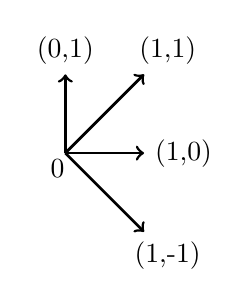
\begin{tikzpicture}[e/.style = {->, line width = 1}]
			\draw[e] (0,0) -- (1,0);
			\draw[e] (0,0) -- (0,1);
			\draw[e] (0,0) -- (1,1);
			\draw[e] (0,0) -- (1,-1);
			\node at (-.1, -.2) {$0$};
			\node at (1.5,0) {(1,0)};
			\node at (1.3,1.3) {(1,1)};
			\node at (0,1.3) {(0,1)};
			\node at (1.3,-1.3) {(1,-1)};
		\end{tikzpicture}
		\caption{Representation by vectors.}
	\end{subfigure}
	\begin{subfigure}{0.45\textwidth}\centering
		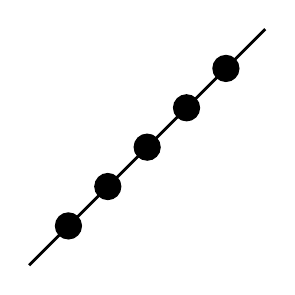
\begin{tikzpicture}[e/.style = {line width = 1}, n/.style = {draw, circle, fill}]
			\draw[e] (0,0) -- (3,3);
			\node[n] at(.5,.5) {};
			\node[n] at(1,1) {};
			\node[n] at(1.5,1.5) {};
			\node[n] at(2,2) {};
			\node[n] at(2.5,2.5) {};
		\end{tikzpicture}
		\caption{Affine representation.}
	\end{subfigure}\\
	\caption{Some different ways of visualization of $U_{2,4}$.}
\end{figure}

Some additional notes are for when we use some other field one can use the Fano's plane which specifically represents a Fano's matroid $F_7$. Which cannot be represented by reals.

\begin{figure}[!ht]\centering
	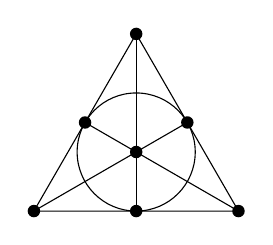
\begin{tikzpicture}[scale=1.5]
	\draw (0,0) circle (0.5);
	\draw (90:1) -- (-30:1)--(210:1)--cycle;
	\draw (90:1)--(0,0);
	\draw (210:1)--(0,0);
	\draw (-30:1)--(0,0);
	\draw (30:0.5)--(0,0);
	\draw (150:0.5)--(0,0);
	\draw (270:0.5)--(0,0);
	\fill (-0.866,-0.5) circle (1.5pt);
	\fill (0.866,-0.5) circle (1.5pt);
	\fill (0,-0.5) circle (1.5pt);
	\fill (0,1) circle (1.5pt);
	\fill (0,0) circle (1.5pt);
	\fill (0.433,0.25) circle (1.5pt);
	\fill (-0.433,0.25) circle (1.5pt);
	\end{tikzpicture}
	\caption{Fano's plane.}
\end{figure}

\section{(Direct) Sum of matroids (also disjoint union)}

\begin{defn}
	We have two matroids $\M_i = (E_i, \I_i)$ for $i= 1,2$, then the (direct) sum $\M_1 \bigoplus \M_2$ is defined as a matroid $\M = (E, \I)$ where $E = E_1 \dot\cup E_2$ and $\I = \{X \subseteq E, X \cap E_i \in \I_i, i=1,2\}$.
\end{defn}

\begin{observ}
	Lets see the basis and circuits:
	
	$$
	\begin{aligned}
		&\B(\M_1 \bigoplus \M_2) = \{B_1 \cup B_2, B_i \in \B_i, i = 1,2\}\\
		&\C(\M_1 \bigoplus \M_2) = \C_1 \cup \C_2\\
		&X \subseteq E : \rank(X) = \rank_1(X \cap E_1) + \rank_2(X \cap E_2)
	\end{aligned}
	$$
\end{observ}